\documentclass[../rapport_MVEX01-11-05]{subfiles}
\begin{document}

\section{Klassificering av hudfärg och urskiljning av händer}\label{sec:hudklassificering}
Det första problemet vid visuell gestigenkänning är att kunna se handen,
och för att kunna göra detta
måste bilden först behandlas. Bildpunkterna måste klassificeras som hud 
eller ickehud, och därefter måste bildområdet med hud i sin tur 
klassificeras som en hand eller som övrig hud.

För att kunna isolera hud i en bild börjar man fördelaktigen med
att transformera bilden till en
lämplig färgrymd, varpå statistiska metoder kan användas för att
markera bildpunkterna som hud respektive ickehud.
Det andra problemet, att identifiera handen bland hudobjekten i bilden kan göras
exempelvis genom subtraktion av objekt som matchar ett ansiktes form, men en enklare
metod är att ta det objekt som ligger längst till vänster i bilden. Denna metod
förklaras mer utförligt i \ref{sec:metod_hud:urskiljning}.

\subsection{Färgrymder}\label{sec:klassificering:fargrymder}
En färg kan matematiskt beskrivas som en vektor i ett färgrum, vars
basvektorer är som grundfärgerna i ett färgsystem.
För att kunna representera alla färger
behöver man ett tredimensionellt färgrum, men i vissa situationer kan
det räcka --- kanske till och med vara fördelaktigt --- med ett
tvådimensionellt färgrum \cite{Kakumanu07}.

Vilken färgrymd som är lämpligast för hudklassificering har inget
entydigt svar.
RGB-färgrymden (röd, grön, blå) har använts av bland annat
\citeasnoun{Lockton02} och \citeasnoun{Sebe04}, och ter sig lämplig
eftersom det är denna färgrymd som används i datorer. Perceptuella
färgrymder, såsom HSL, separerar kulör, mättnad och ljusintensitet.
De har inte rönt någon större framgång dels då deras definierande
transformationer innehåller singulariteter, dels då de är
prestandamässigt ofördelaktiga.

Ortogonala färgrymder har däremot nått utbredd användning för
hudklassificering \cite{Hsu02,Elmezain08,Hassanpour08} eftersom de
både separerar kulör och mättnad från ljusstyrka, och är affina avbildningar av
RGB. 
En ortogonal färgrymd som har visat sig särskiljt bra är $YC_bC_r$ \cite{Kakumanu07}.

\subsection[Färgrymden $\mathrm{YC_bC_r}$]{Färgrymden $\mathbf{YC_bC_r}$}
$YC_bC_r$-rymden är en ortogonalisering av RGB-rymden genom en
affin transformation, vilken resulterar i en basvektor som
representerar ljusstyrka ($Y$) och två som representerar färg (chroma), $C_b$ och $C_r$. Enligt
internationell standard \cite{ITU-BT601} ges
transformationen av
\begin{equation*}
  \label{eq:farg:ycbcr}
  \begin{gathered}
  Y   = 16  + ( 65.481R + 128.553G + 24.966B)\\
  C_b = 128 + (-37.797R - 74.203G  + 112.0B )\\
  C_r = 128 + (112.0R   - 93.786G  - 18.214B)
  \end{gathered}
\end{equation*}
där $R$, $G$, och $B$ är värden mellan $0$ och $255$ som representerar
färgens värde i RGB-rymden.

\subsection{Sannolikhetsfördelning för hudfärg}\label{sec:klassificering:hud}

För att skilja bildpunkter med hud från bakgrunden,
kan flera olika statistiska metoder
appliceras. Man har till exempel gjort försök med skogar av
slumpmässiga träd
\cite{Khan10}, Bayesiska nätverk \cite{Sebe04}, generativa modeller
\cite{Kruppa02}
och luddig aritmetik \cite{Shang10} --- en större undersökning av metoder
för huddetektion gjordes av \citeasnoun{Kakumanu07}.

En enklare metod som nått relativt stor framgång är den som baseras på
Gaussian Mixture Models \cite{Elmezain08,Hassanpour08}, det vill säga
en modell där bildpunktens färg antas bero stokastiskt på om
bildpunkten föreställer hud eller inte.

Färgen antas då vara en multivariat normalfördelad
stokastisk variabel, där fördelningens parametrar beror på om
bildpunkten motsvarar hud eller inte. För att kunna hantera olika hudfärger kan en
uppsättning av olika
fördelningar för respektive hudfärg användas. Den totala
sannolikhetsfördelning är sedan en linjärkombination av dessa. Detsamma
kan göras med sannolikhetsfördelningen för bildpunkter som inte
innehåller hud.

För att bestämma väntevärdesvektorn och kovariansmatrisen i en
uppskattad normalfördelning krävs ett
antal datapunkter, med vilkas hjälp parametrarna kan skattas med maximum
likelihood-metoden.

Fördelningen ges allmänt av
\begin{equation*}
  p(x)=\frac{1}{(2\pi)^{d/2}|\Sigma|^{1/2}}e^{-(\vect{x}-\mu)^T\Sigma^{-1}(\vect{x}-\mu)/2},
\end{equation*}
där $\mu$ är väntevärdesvektorn och $\Sigma$ är kovariansmatrisen, definierad
genom sina element
\begin{equation*}
 \sigma_{i,j}=\text{Cov}[X_1,X_2]=\text{E}[(X_1-\mu_1)(X_2-\mu_2)]].
\end{equation*}
\notes{index, 1/2 eller i/j?}

Med N datapunkter fås de skattade parametrarna

\begin{gather*}
  \hat\mu    =\frac{1}{N}\sum_{i=1}^N\vect{x}_i\\
  \hat\Sigma =\frac{1}{N-1}\sum_{i=1}^N(\vect{x}_i-\hat\mu)(\vect{x}_i-\hat\mu)^T
\end{gather*}

För att ytterligare förbättra fördelningarna kan de antas vara
en linjärkombination av flera normalfördelningar. En iterativ metod för optimering av
sådana fördelningar beskrivs av \citeasnoun{Elmezain08}.

För varje bildpunktsfärg kan med dessa fördelningar sannolikheten för att färgen ska
förekomma då bildpunkten föreställer hud
respektive ickehud bestämmas. Det är rimligt att klassa en bildpunkt som
hud om sannolikheten för att bildpunkten föreställer hud är större än
sannolikheten att den inte gör det givet dess färg, dvs.~om
\begin{equation*}
	\frac{\Prob(\textrm{hud}|\textrm{färg})}{\Prob(\textrm{ickehud}|\textrm{färg})} > 1.
\end{equation*}

Ibland kan det vara önskvärt att kräva att kvoten ska vara ännu
större, då det är värre att klassa ickehud som hud (och då lägga
handen i det som egentligen är bakgrund) än att klassa hud som ickehud
(och få en för liten hand). Man ställer därför istället kravet 
\begin{equation*}
	\frac{\Prob(\textrm{hud}|\textrm{färg})}{\Prob(\textrm{ickehud}|\textrm{färg})} > c,
\end{equation*}
där konstanten $c$ anpassas för att få så bra resultat som möjligt.

De sannolikheter som kan bestämmas med de skattade parametrarna från den
multivariata distributionen är
$\Prob(\textrm{färg}|\textrm{hud})$ och
$\Prob(\textrm{färg}|\textrm{ickehud})$. Med hjälp av Bayes sats
kan kvoten ovan omformuleras enligt
\begin{multline*}
\frac{\Prob(\textrm{hud}|\textrm{färg})}{\Prob(\textrm{ickehud}|\textrm{färg})}=\\
=\frac{\Prob(\textrm{färg}|\textrm{hud})\Prob(\textrm{hud})}{\Prob(\textrm{färg})}
 \frac{\Prob(\textrm{färg}}{\Prob(\textrm{ickehud})\Prob(\textrm{ickehud}|\textrm{färg})}=\\
=\frac{\Prob(\textrm{färg}|\textrm{hud})\Prob(\textrm{hud})}{\Prob(\textrm{färg}|\textrm{ickehud})
 \Prob(\textrm{ickehud})},
\end{multline*}
och på så sätt kan man använda tidigare nämnda distributioner för att
klassificera hud i bilden. 

Kvoten $\Prob(\textrm{hud})/\Prob(\textrm{ickehud})$ måste uppskattas och betecknar
den förväntade mängden hudbildpunkter i bilden genom den förväntade mängden
ickehudbildpunkter. Denna kvot kan bakas in i konstanten $c$, och vi
får vårt slutliga krav för att klassa en bildpunkt som hud:

\begin{equation*}
	\frac{\Prob(\textrm{färg}|\textrm{hud})}{\Prob(\textrm{färg}|\textrm{ickehud})} > c,
\end{equation*}

där $c$ anpassas separat. På detta sätt kan en bild från kameran göras
binär, varje bildpunkt är antingen hud eller ickehud.

Denna metod för att klassa bildpunkter leder dock till att en del
bildpunkter klassas fel, vilket resulterar i svarta öar i handen
och vita öar i bakgrunden. För att bli av med dessa används
morfologiska operationer.

\subsection{Morfologiska operationer}\label{sec:morph}

\begin{figure}[tb]
	\centering 
	\subfloat[Originalbilden]{
		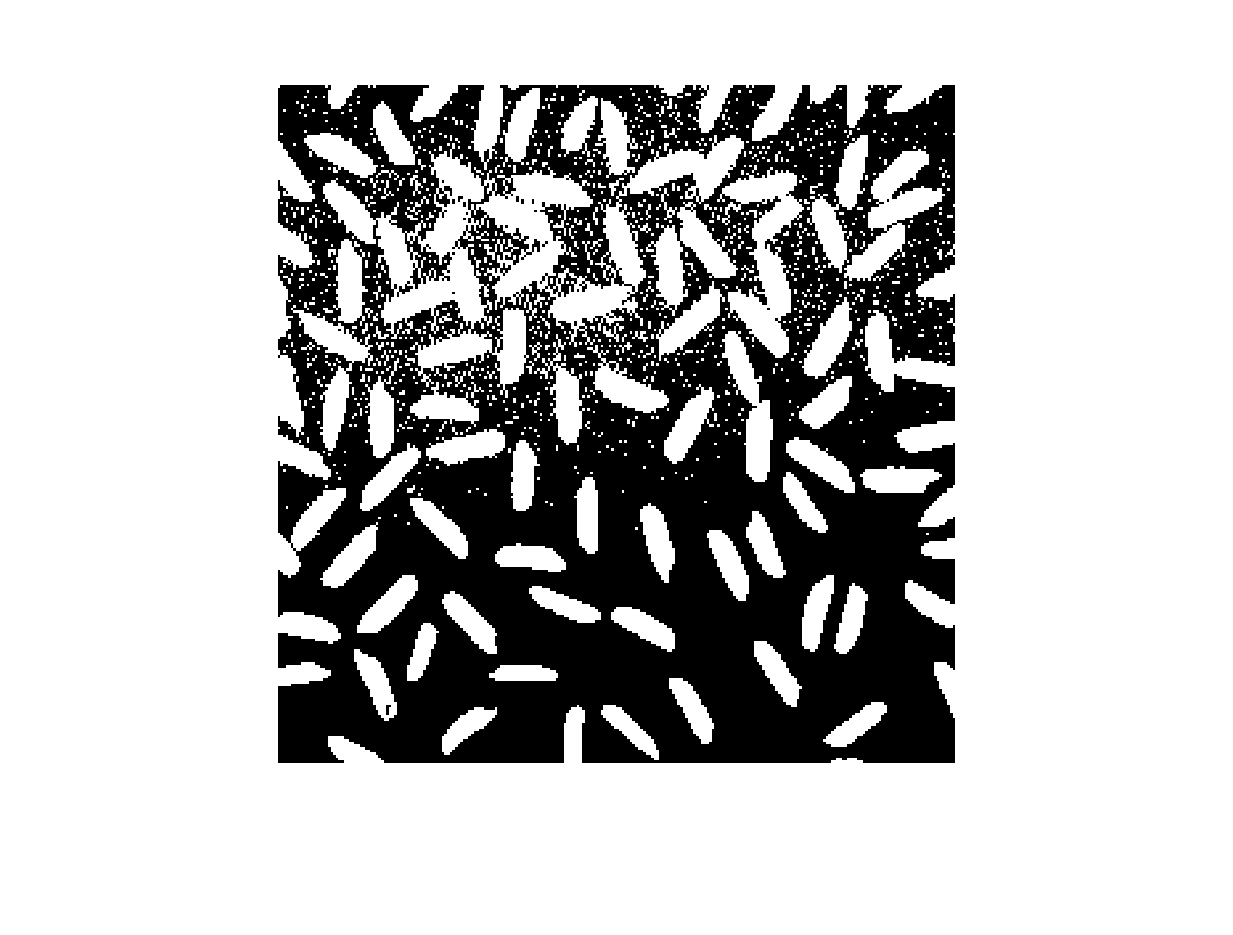
\includegraphics[width=0.3\textwidth,trim=115 75 115 20,clip=true]{bilder/morph-orig}
		\label{fig:morph:or}
	}
	\subfloat[Erosion]{
		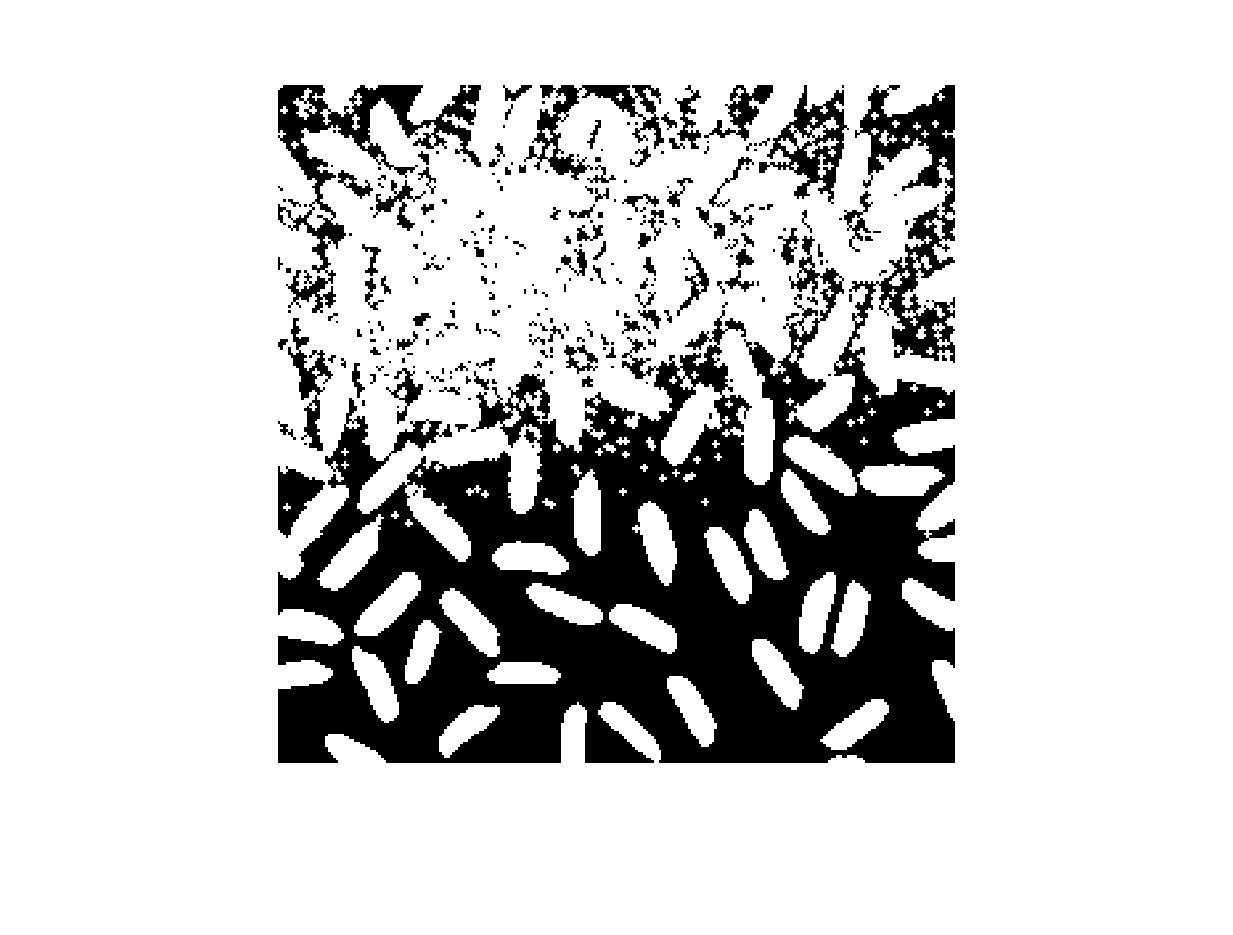
\includegraphics[width=0.3\textwidth,trim=115 75 115 20,clip=true]{bilder/morph-erosion}
 		\label{fig:morph:er}
	}
	\subfloat[Dilatation]{
		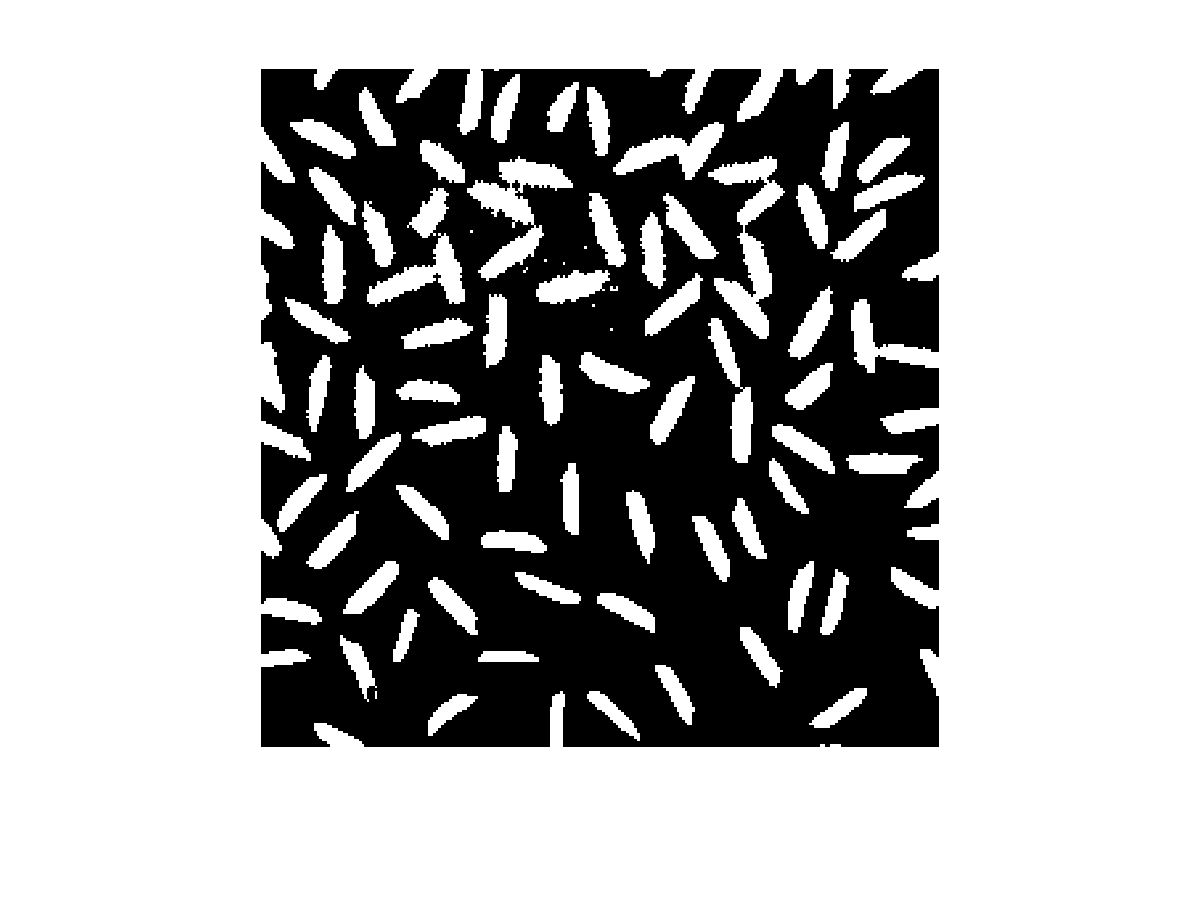
\includegraphics[width=0.3\textwidth,trim=115 75 115 20,clip=true]{bilder/morph-dilatation}
		\label{fig:morph:di}
	}
	\\
	\hspace{0.3\textwidth}\quad % ser det fult ut kanske?
	\subfloat[Öppning]{
		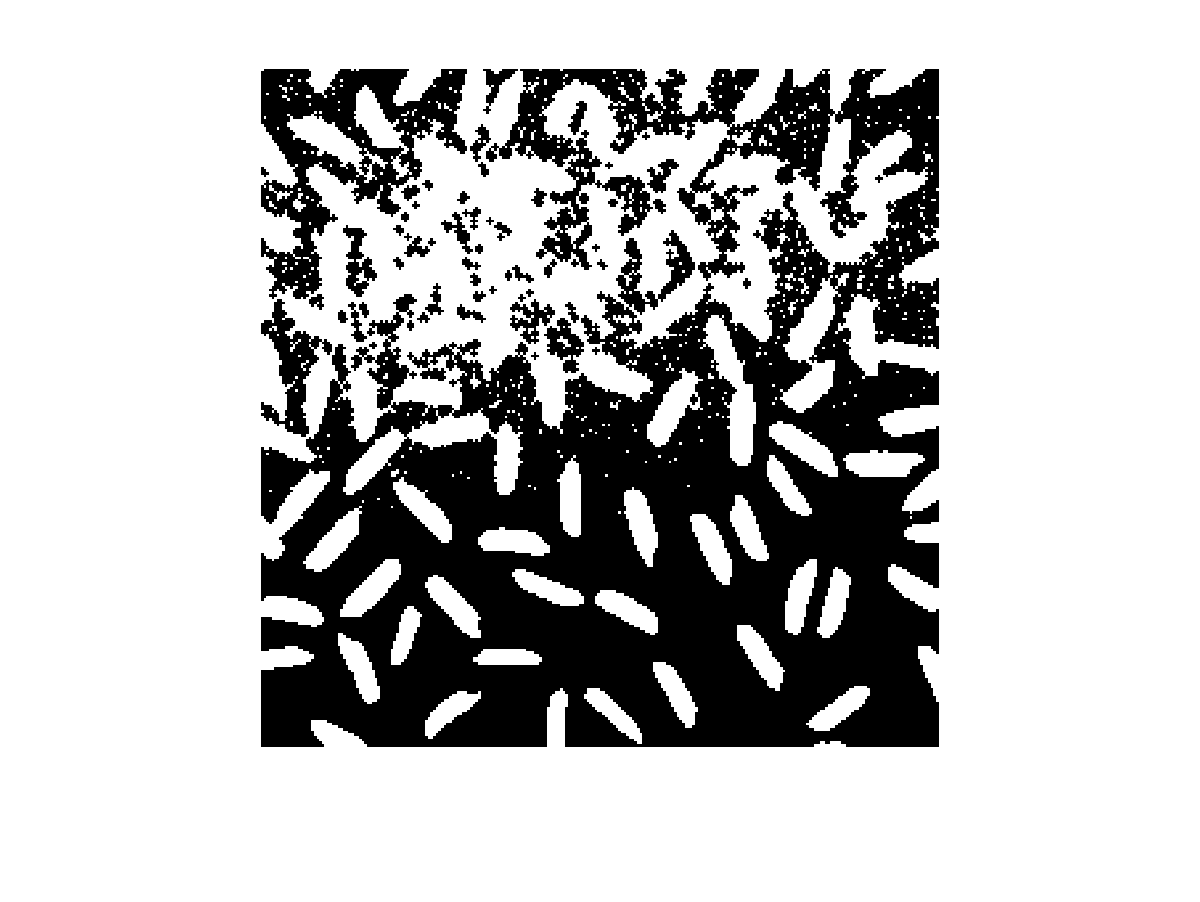
\includegraphics[width=0.3\columnwidth,trim=115 75 115 20,clip=true]{bilder/morph-oppning}
		\label{fig:morph:op}
	}
	\subfloat[Stängning]{
		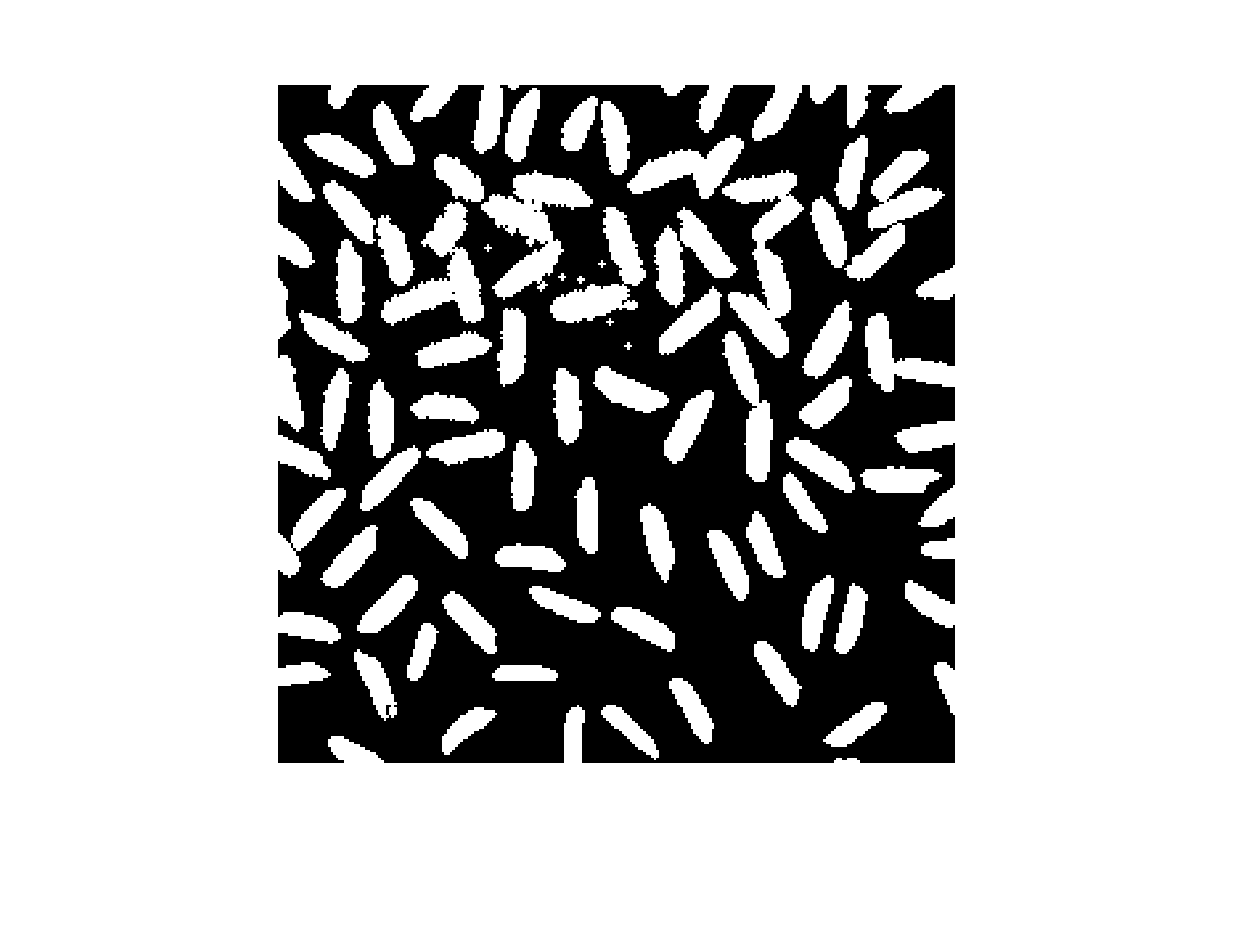
\includegraphics[width=0.3\columnwidth,trim=115 75 115 20,clip=true]{bilder/morph-stangning}
		\label{fig:morph:cl}
	}
	\caption{De fyra morfologiska operationerna}
	\label{fig:morph}
\end{figure}

Morfologiska operationer kan användas för att modifiera områden i
binära bilder, till exempel för att rensa bort brus eller för att
mjuka upp kanter. Det finns fyra grundläggande morfologiska
operationer: \emph{erosion}, \emph{dilatation}, \emph{öppning} och
\emph{stängning} \cite[s.~25]{Rudemo09}, vars resultat visas i figur~\ref{fig:morph}.

Dessa definieras som operationer på mängder; specifikt mängden $A$
av alla svarta bildpunkter i bilden vi behandlar, dvs. alla bildpunkter som är
''avstängda'' och mängden $S$ som representerar ett strukturelement
som i någon mening förändrar hur operationen verkar på bilden.
Strukturelementet kan dessutom förflyttas så att dess referensbildpunkt
ligger på plats $(i,j)$ i bilden --- kalla detta förflyttade
strukturelement för $S_{i,j}$. Innebörden av $S$ framgår ur hur det används
nedan.

\emph{Erosionen} eroderar bort delar av de svarta områdena genom
att endast behålla de bildpunkter vars ''omgivning'' (definierad av mängden
$S_{i,j}$) ligger helt i mängden $A$. Vad operationen egentligen gör är alltså
att skala av det yttersta lagret, randen, av mängden $A$. Erosion definieras enligt
\begin{equation*}
  A\ominus S = \{(i,j)\;:\;S_{i,j}\subseteq A\}.
\end{equation*}

Dess motsats, \emph{dilatation}, agerar som
en erosion på komplementet till $A$ och definieras enligt
\begin{equation*}
  A\oplus S = (A^C\ominus S)^C.
\end{equation*}

Dessa operationer är i sig inte särskilt användbara då de förändrar
arean av objektet i bilderna. Operationerna kan dock kombineras för
att skapa operationer som i någon mening endast 
''mjukar upp'' objektet i bilden utan att förändra deras area markant.
Eftersom erosion och dilatation är motsatser kan dessa appliceras i
följd för att behandla bilden och
sedan återställa den. Detta ger upphov till två nya operationer:
\emph{öppning} och \emph{stängning}.

En öppning är en erosion följd av en dilatation, enligt
\begin{equation*}
  \phi_S(A)=(A\ominus S)\oplus S'.
\end{equation*}

Detta resulterar i att svart brus, dvs.~svarta områden som inte kan täckas
av $S$, försvinner i
första steget varefter större svarta områdena utökas till sin ursprungliga
storlek i det andra
steget. Operationen ''öppnar upp'' vita områden.

En stängning består av den omvända proceduren, enligt
\begin{equation*}
  \Phi_S(A)=(A\oplus S)\ominus S',
\end{equation*}
och ger även motsatt resultat (svarta områden ''öppnas upp'').

De
båda operationerna använder utöver $A$ och $S$ även $S'$, vilket är
$S$ roterad 180\textdegree{} runt sin referensbildpunkt.

\end{document} 
